

\tikzset{every picture/.style={line width=0.75pt}} %set default line width to 0.75pt        

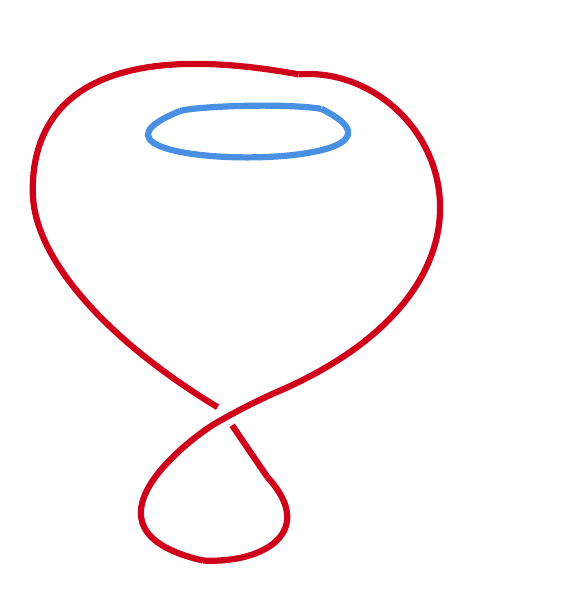
\begin{tikzpicture}[x=0.75pt,y=0.75pt,yscale=-1,xscale=1]
%uncomment if require: \path (0,300); %set diagram left start at 0, and has height of 300

%Curve Lines [id:da2574706672222027] 
\draw [color={rgb, 255:red, 208; green, 2; blue, 27 }  ,draw opacity=1 ][line width=2.25]    (343,46.68) .. controls (407,41.68) and (460,141.77) .. (337,197.77) ;
%Curve Lines [id:da15123885693185346] 
\draw [color={rgb, 255:red, 208; green, 2; blue, 27 }  ,draw opacity=1 ][line width=2.25]    (337,197.77) .. controls (324.03,203.31) and (311.19,209.93) .. (302.21,215.27) .. controls (293.23,220.61) and (231,265.75) .. (297,280.92) ;
%Curve Lines [id:da3972148663663959] 
\draw [color={rgb, 255:red, 208; green, 2; blue, 27 }  ,draw opacity=1 ][line width=2.25]    (343,46.68) .. controls (228,25.68) and (214,74.97) .. (215,104.68) .. controls (216,134.4) and (248,173.03) .. (304,207.03) ;
%Curve Lines [id:da738003714112636] 
\draw [color={rgb, 255:red, 208; green, 2; blue, 27 }  ,draw opacity=1 ][line width=2.25]    (328,240.75) .. controls (352,266.75) and (326.73,282.41) .. (297,280.92) ;
%Straight Lines [id:da4622187536301742] 
\draw [color={rgb, 255:red, 208; green, 2; blue, 27 }  ,draw opacity=1 ][fill={rgb, 255:red, 208; green, 2; blue, 27 }  ,fill opacity=1 ][line width=2.25]    (311,215.75) -- (328,240.75) ;
%Curve Lines [id:da6698966779960203] 
\draw [color={rgb, 255:red, 74; green, 144; blue, 226 }  ,draw opacity=1 ][line width=2.25]    (286,64.3) .. controls (214,93.3) and (419,95.3) .. (354,63.3) ;
%Curve Lines [id:da9780890335727794] 
\draw [color={rgb, 255:red, 74; green, 144; blue, 226 }  ,draw opacity=1 ][line width=2.25]    (286,64.3) .. controls (293,62.18) and (335,60.3) .. (354,63.3) ;




\end{tikzpicture}
